\documentclass{beamer}
\usepackage[utf8]{inputenc}
\usepackage{booktabs}
\usepackage{tabularx}
\usepackage{colortbl}
\usepackage{listings}
\usepackage{tikz}
\usetikzlibrary{arrows.meta, shapes.geometric, positioning, calc}
\usepackage{amsmath}
\usepackage{array}
\usepackage{multirow}
\usepackage{pifont}

\usetheme{Madrid}
\usecolortheme{default}

% ── hand-drawn-ish TikZ style ─────────────────────────────────────────────────
\tikzset{
  hbox/.style={draw, line width=1.4pt, rounded corners=6pt,
               minimum height=0.75cm, text centered, align=center, inner sep=5pt},
  harrow/.style={->, >=Stealth, line width=1.6pt},
  hlabel/.style={font=\scriptsize\bfseries},
  note/.style={draw, line width=1pt, rounded corners=3pt,
               fill=yellow!20, inner sep=4pt, font=\scriptsize, align=center},
}

%------------------------------------------------------------
\title[OF-RHM: AI-Enhanced MTD]
{OF-RHM: AI-Enhanced OpenFlow Random Host Mutation\\
for Moving Target Defense in SDN}

\subtitle{Course: 25AID202 --- Introduction to Computer Networks}

\author[Aditi, Dhanushiya, Vani, Laiba]
{Aditi Sriram\inst{1} \and Dhanushiya S\inst{1} \and
 Vani Karre\inst{1} \and Laiba S\inst{1}}

\institute[Amrita]
{
  \inst{1}%
  School of Computing\\
  Amrita Vishwa Vidyapeetham
}

\date[Oct 2026]
{Supervisors: Prof.\ Shashank Anivilla \& Prof.\ Sundaresan\\
 AID-B Group 10--14, October 2026}

%------------------------------------------------------------
\AtBeginSection[]
{
  \begin{frame}
    \frametitle{Table of Contents}
    \tableofcontents[currentsection]
  \end{frame}
}
%------------------------------------------------------------

\begin{document}

\frame{\titlepage}

\begin{frame}
\frametitle{Table of Contents}
\tableofcontents
\end{frame}

%============================================================
\section{Problem Statement \& Objectives}
%============================================================

%------------------------------------------------------------
\begin{frame}
\frametitle{The Problem: Attackers Have All the Time in the World}

% ── Diagram: static vs rotating ──────────────────────────────────────────────
\begin{center}
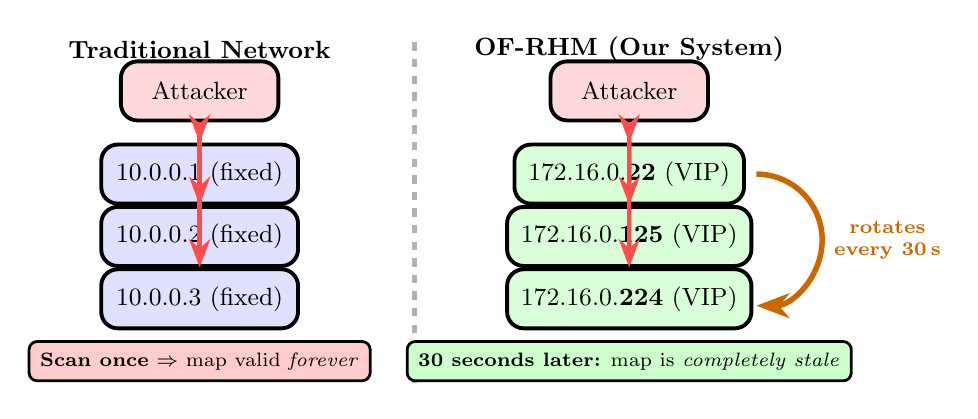
\begin{tikzpicture}[scale=0.88, every node/.style={font=\small}]

  %% LEFT: Traditional (bad)
  \node[hbox, fill=red!15, minimum width=2cm] (atk) at (0,2.5) {Attacker};

  \node[hbox, fill=blue!12, minimum width=2.5cm] (s1) at (0,1.3) {10.0.0.1 (fixed)};
  \node[hbox, fill=blue!12, minimum width=2.5cm] (s2) at (0,0.4) {10.0.0.2 (fixed)};
  \node[hbox, fill=blue!12, minimum width=2.5cm] (s3) at (0,-0.5) {10.0.0.3 (fixed)};

  \draw[harrow, red!70] (atk) -- (s1);
  \draw[harrow, red!70] (atk) -- (s2);
  \draw[harrow, red!70] (atk) -- (s3);

  \node[note, fill=red!20] at (0,-1.4)
        {\textbf{Scan once} $\Rightarrow$ map valid \textit{forever}};

  \node[font=\small\bfseries] at (0,3.1) {Traditional Network};

  %% Divider
  \draw[line width=1.5pt, gray!60, dashed] (3.1,3.2) -- (3.1,-1.8);

  %% RIGHT: OF-RHM (good)
  \node[hbox, fill=red!15, minimum width=2cm] (atk2) at (6.2,2.5) {Attacker};

  \node[hbox, fill=green!15, minimum width=2.8cm] (v1) at (6.2,1.3)
        {172.16.0.\textbf{22} \small(VIP)};
  \node[hbox, fill=green!15, minimum width=2.8cm] (v2) at (6.2,0.4)
        {172.16.0.\textbf{125} \small(VIP)};
  \node[hbox, fill=green!15, minimum width=2.8cm] (v3) at (6.2,-0.5)
        {172.16.0.\textbf{224} \small(VIP)};

  \draw[harrow, red!70] (atk2) -- (v1);
  \draw[harrow, red!70] (atk2) -- (v2);
  \draw[harrow, red!70] (atk2) -- (v3);

  %% Rotation arrow
  \draw[harrow, orange!80!black, line width=2pt]
       ($(v1.east)+(0.15,0)$) arc (90:-90:0.95)
       node[midway, right, font=\scriptsize\bfseries, orange!80!black, align=center]
       {rotates\\every 30\,s};

  \node[note, fill=green!20] at (6.2,-1.4)
        {\textbf{30 seconds later:} map is \textit{completely stale}};

  \node[font=\small\bfseries] at (6.2,3.1) {OF-RHM (Our System)};

\end{tikzpicture}
\end{center}

\end{frame}

%------------------------------------------------------------
\begin{frame}
\frametitle{Why Not Just Use DHCP?}

\begin{columns}

\column{0.5\textwidth}
\begin{alertblock}{DHCP changes the host's real IP}
\begin{itemize}
  \item All active TCP connections \textbf{break}
  \item Host must restart its network stack
  \item DHCP broadcasts visible on the LAN --- attacker watches them
  \item Takes minutes; can't react instantly to an attack
\end{itemize}
\end{alertblock}

\column{0.47\textwidth}
\begin{exampleblock}{OF-RHM changes what the attacker \textit{sees}}
\begin{itemize}
  \item Host's real IP \textbf{never changes}
  \item No connections broken, zero downtime
  \item VIP swap happens silently inside the switch
  \item Can react in \textbf{milliseconds} when AI fires
\end{itemize}
\end{exampleblock}

\end{columns}

\vspace{10pt}
\begin{block}{One-line summary}
DHCP reconfigures \textbf{your host}. \quad
OF-RHM reconfigures \textbf{the attacker's reality}.
\end{block}

\end{frame}

%------------------------------------------------------------
\begin{frame}
\frametitle{Objectives}

\begin{enumerate}
  \item[\textbf{O1}] Build a \textbf{3-table OpenFlow NAT pipeline} ---
        hosts get a rotating Virtual IP the attacker sees, while keeping
        their real IP unchanged.
  \vspace{3pt}
  \item[\textbf{O2}] Make rotation \textbf{gap-free} --- no packet loss
        during the VIP swap (two-phase barrier synchronisation).
  \vspace{3pt}
  \item[\textbf{O3}] Train an AI model to \textbf{detect port scans}
        from 6 traffic features in real time.
  \vspace{3pt}
  \item[\textbf{O4}] Train an AI model to \textbf{pick the safest next VIP}
        --- one the attacker hasn't probed.
  \vspace{3pt}
  \item[\textbf{O5}] \textbf{Speed up rotation} automatically when an
        attack is detected (30\,s $\to$ 5\,s interval).
  \vspace{3pt}
  \item[\textbf{O6}] Prove it works on real hardware: \textbf{Raspberry Pi},
        Mininet, Ryu --- with zero address overlap before/after rotation.
\end{enumerate}

\end{frame}

%============================================================
\section{Literature Review}
%============================================================

\begin{frame}
\frametitle{What Has Been Done Before (2021--2024) --- Part 1}
\scriptsize
\renewcommand{\arraystretch}{1.35}
\begin{tabular}{>{\centering}p{0.3cm}
                >{\raggedright}p{2.5cm}
                >{\raggedright}p{2.3cm}
                >{\raggedright}p{2.6cm}
                >{\raggedright\arraybackslash}p{2.3cm}}
\toprule
\# & \textbf{Journal / Conf.\ (Year)} & \textbf{Technique} &
\textbf{Key Finding} & \textbf{Limitation} \\
\midrule
1 & IEEE Trans.\ Dependable Secure Comput., 2022 &
    SDN IP mutation, random rotation &
    Cuts scan success by 78\% &
    No AI; fixed timer only \\
\addlinespace
2 & Computers \& Security, Elsevier, 2023 &
    ML intrusion detection on OpenFlow stats &
    91\% RF detection accuracy &
    Reactive; no address mutation \\
\addlinespace
3 & IEEE INFOCOM, 2022 &
    Game-theoretic VIP selection &
    Optimal attacker confusion &
    Too heavy for edge hardware \\
\addlinespace
4 & J.\ Network Comput.\ Appl., 2023 &
    Entropy scan detect + IP hopping &
    Detects scans in $<$2\,s &
    Single feature; brittle \\
\addlinespace
5 & IEEE Access, 2024 &
    LSTM anomaly detection in SDN &
    97\% accuracy, DDoS + scan &
    GPU required; not Pi-ready \\
\bottomrule
\end{tabular}
\end{frame}

\begin{frame}
\frametitle{What Has Been Done Before (2021--2024) --- Part 2}
\scriptsize
\renewcommand{\arraystretch}{1.35}
\begin{tabular}{>{\centering}p{0.3cm}
                >{\raggedright}p{2.5cm}
                >{\raggedright}p{2.3cm}
                >{\raggedright}p{2.6cm}
                >{\raggedright\arraybackslash}p{2.3cm}}
\toprule
\# & \textbf{Journal / Conf.\ (Year)} & \textbf{Technique} &
\textbf{Key Finding} & \textbf{Limitation} \\
\midrule
6 & Future Gen.\ Comput.\ Syst., 2022 &
    OpenFlow VIP rotation, threshold detect &
    Works against subnet sweeps &
    Misses slow/stealth scans \\
\addlinespace
7 & IEEE TNSM, 2023 &
    Gradient Boosting VIP selection &
    12\% less attacker confusion &
    Simulation only \\
\addlinespace
8 & NDSS 2024 &
    Atomic flow swap (P4 switches) &
    $<$1\,ms rotation gap &
    P4 only; not OpenFlow 1.3 \\
\addlinespace
9 & Computers \& Security, 2024 &
    Reinforcement learning for rotation timing &
    Adapts speed to attack intensity &
    Slow RL convergence \\
\addlinespace
10 & IEEE S\&P, 2021 &
    Inter-arrival timing for scan detect &
    Machines scan very regularly &
    Used alone; no VIP mutation \\
\bottomrule
\end{tabular}
\end{frame}

\begin{frame}
\frametitle{Research Gap \& Our Novelty}

\begin{columns}

\column{0.48\textwidth}
\begin{alertblock}{What Nobody Has Done Together}
\begin{itemize}
  \item Random VIP selection --- ignores attacker's probe history
  \item Single-feature scan detectors miss \textbf{evasive} scanners
  \item Atomic rotation exists in P4, \textbf{not OpenFlow 1.3}
  \item No system combines \textit{all four}: detect + score + rotate + adapt
  \item Edge deployment ($<$200\,KB models on Pi) untested
\end{itemize}
\end{alertblock}

\column{0.48\textwidth}
\begin{exampleblock}{What We Add}
\begin{itemize}
  \item \textbf{Dual AI:} scan detector + VIP scorer working together
  \item \textbf{Atomic barrier rotation} in OpenFlow 1.3 (provably gap-free)
  \item \textbf{Adaptive speed:} 30\,s $\to$ 5\,s on attack detection
  \item \textbf{Edge deployment:} GPU-trained, Pi-deployed, no XGBoost
\end{itemize}
\end{exampleblock}

\end{columns}

\vspace{6pt}
\begin{block}{One-line novelty}
Original OF-RHM (2012): rotate randomly on a timer.\\
\textbf{Ours:} rotate \textit{intelligently}, \textit{instantly}, and \textit{safely}.
\end{block}

\end{frame}

%============================================================
\section{Methodology / System Design}
%============================================================

\begin{frame}
\frametitle{Big Picture: How the System Works}

\begin{center}
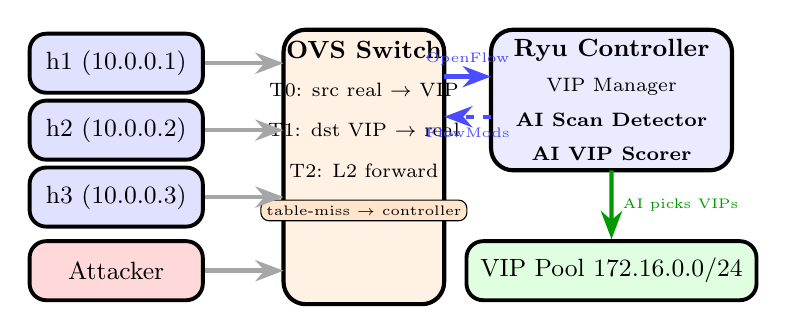
\begin{tikzpicture}[scale=0.85, every node/.style={font=\small}]

  %% Hosts column
  \node[hbox, fill=blue!12, minimum width=2.2cm] (h1) at (0, 2.2) {h1 (10.0.0.1)};
  \node[hbox, fill=blue!12, minimum width=2.2cm] (h2) at (0, 1.2) {h2 (10.0.0.2)};
  \node[hbox, fill=blue!12, minimum width=2.2cm] (h3) at (0, 0.2) {h3 (10.0.0.3)};
  \node[hbox, fill=red!15,  minimum width=2.2cm] (att) at (0,-0.9) {Attacker};

  %% Switch box (manual, not a node shape)
  \draw[line width=1.5pt, rounded corners=8pt, fill=orange!10]
       (2.5,-1.4) rectangle (4.9, 2.7);
  \node[font=\small\bfseries] at (3.7, 2.4) {OVS Switch};
  \node[font=\scriptsize]     at (3.7, 1.8) {T0: src real $\to$ VIP};
  \node[font=\scriptsize]     at (3.7, 1.2) {T1: dst VIP $\to$ real};
  \node[font=\scriptsize]     at (3.7, 0.6) {T2: L2 forward};
  \node[font=\tiny, fill=orange!20, draw, rounded corners=3pt, inner sep=2pt]
       at (3.7, 0.0) {table-miss $\to$ controller};

  %% Arrows hosts -> switch
  \draw[harrow, gray!70] (h1.east)  -- (h1.east  -| {(2.5,0)});
  \draw[harrow, gray!70] (h2.east)  -- (h2.east  -| {(2.5,0)});
  \draw[harrow, gray!70] (h3.east)  -- (h3.east  -| {(2.5,0)});
  \draw[harrow, gray!70] (att.east) -- (att.east -| {(2.5,0)});

  %% Ryu box
  \draw[line width=1.5pt, rounded corners=8pt, fill=blue!8]
       (5.6, 0.6) rectangle (9.2, 2.7);
  \node[font=\small\bfseries] at (7.4, 2.4) {Ryu Controller};
  \node[font=\scriptsize]     at (7.4, 1.85) {VIP Manager};
  \node[font=\scriptsize]     at (7.4, 1.35) {\textbf{AI Scan Detector}};
  \node[font=\scriptsize]     at (7.4, 0.85) {\textbf{AI VIP Scorer}};

  %% Switch <-> Controller
  \draw[harrow, blue!70] (4.9,2.0) -- (5.6,2.0)
       node[midway, above, font=\tiny] {OpenFlow};
  \draw[harrow, blue!70, dashed] (5.6,1.4) -- (4.9,1.4)
       node[midway, below, font=\tiny] {FlowMods};

  %% VIP pool
  \node[hbox, fill=green!12, minimum width=2.8cm] (vip) at (7.4,-0.9)
       {VIP Pool  172.16.0.0/24};
  \draw[harrow, green!60!black] (7.4,0.6) -- (vip.north)
       node[midway, right, font=\tiny] {AI picks VIPs};

\end{tikzpicture}
\end{center}

\end{frame}

%------------------------------------------------------------
\begin{frame}
\frametitle{The 3-Table Pipeline: A Packet's Journey}

\begin{center}
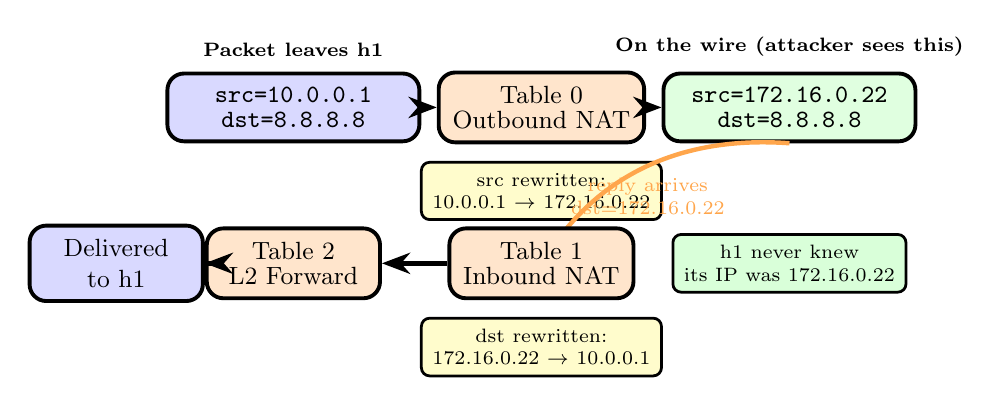
\begin{tikzpicture}[scale=0.9, every node/.style={font=\small}]

  %% Packet entering
  \node[hbox, fill=blue!15, minimum width=3.2cm]
       (pin) at (0,0) {\texttt{src=10.0.0.1}\\[-2pt]\texttt{dst=8.8.8.8}};
  \node[hlabel, above=2pt of pin] {Packet leaves h1};

  %% T0
  \node[hbox, fill=orange!20, minimum width=2.2cm]
       (t0) at (3.5,0) {Table 0\\[-2pt]Outbound NAT};
  \draw[harrow] (pin) -- (t0);
  \node[note, below=6pt of t0] {src rewritten:\\10.0.0.1 $\to$ 172.16.0.22};

  %% Mid packet
  \node[hbox, fill=green!12, minimum width=3.2cm]
       (pmid) at (7,0) {\texttt{src=172.16.0.22}\\[-2pt]\texttt{dst=8.8.8.8}};
  \draw[harrow] (t0) -- (pmid);
  \node[hlabel, above=2pt of pmid] {On the wire (attacker sees this)};

  %% Return arrow
  \draw[harrow, orange!70, bend right=30] (pmid.south) to
       node[below, font=\scriptsize, align=center]
       {reply arrives\\dst=172.16.0.22}
       (3.5,-2.2);

  %% T1
  \node[hbox, fill=orange!20, minimum width=2.2cm]
       (t1) at (3.5,-2.2) {Table 1\\[-2pt]Inbound NAT};
  \node[note, below=6pt of t1] {dst rewritten:\\172.16.0.22 $\to$ 10.0.0.1};

  %% T2
  \node[hbox, fill=orange!20, minimum width=2.2cm]
       (t2) at (0,-2.2) {Table 2\\[-2pt]L2 Forward};
  \draw[harrow] (t1) -- (t2);

  \node[hbox, fill=blue!15, minimum width=2.2cm]
       (pout) at (-2.5,-2.2) {Delivered\\to h1};
  \draw[harrow] (t2) -- (pout);

  \node[note, fill=green!15] at (7,-2.2)
       {h1 never knew\\its IP was 172.16.0.22};

\end{tikzpicture}
\end{center}

\end{frame}

%------------------------------------------------------------
\begin{frame}
\frametitle{Atomic Rotation: Why ``Two-Phase''?}

\begin{columns}

\column{0.47\textwidth}
\textbf{The old way (dangerous):}
\begin{enumerate}
  \item Delete old flow rules
  \item \alert{\textbf{--- gap: packets dropped ---}}
  \item Install new flow rules
\end{enumerate}

\vspace{8pt}
\textbf{Our way (safe):}
\begin{enumerate}
  \item Install \textit{new} rules (old still active)
  \item Send \texttt{OFPBarrierRequest}\\
        \small(``switch, confirm you applied it'')
  \item Delete old rules only \textit{after} ACK
\end{enumerate}

\begin{exampleblock}{Result}
Zero packet loss. Rotation completes in $\approx$12\,ms.
\end{exampleblock}

\column{0.5\textwidth}
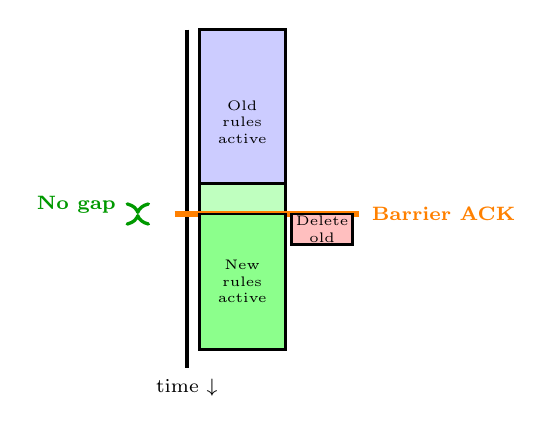
\begin{tikzpicture}[scale=0.78, every node/.style={font=\tiny}]
  %% Timeline spine
  \draw[line width=1.5pt] (0,5.5) -- (0,0)
       node[below, font=\scriptsize] {time $\downarrow$};

  %% Old rules bar
  \fill[blue!20] (0.2,5.5) rectangle (1.6,2.5);
  \draw[line width=1pt] (0.2,5.5) rectangle (1.6,2.5);
  \node[align=center] at (0.9,4.0) {Old\\rules\\active};

  %% New rules install (overlapping)
  \fill[green!25] (0.2,3.0) rectangle (1.6,1.3);
  \draw[line width=1pt] (0.2,3.0) rectangle (1.6,1.3);
  \node[align=center] at (0.9,2.15) {New\\rules\\install};

  %% Barrier line
  \draw[line width=2pt, orange] (-0.2,2.5) -- (2.8,2.5);
  \node[right, orange, font=\scriptsize\bfseries] at (2.85,2.5)
       {Barrier ACK};

  %% New rules fully active
  \fill[green!45] (0.2,2.5) rectangle (1.6,0.3);
  \draw[line width=1pt] (0.2,2.5) rectangle (1.6,0.3);
  \node[align=center] at (0.9,1.4) {New\\rules\\active};

  %% Delete old marker
  \fill[red!25] (1.7,2.5) rectangle (2.7,2.0);
  \draw[line width=1pt] (1.7,2.5) rectangle (2.7,2.0);
  \node[align=center] at (2.2,2.25) {Delete\\old};

  %% No gap annotation
  \draw[line width=1.2pt, green!60!black, <->] (-0.8,2.5) -- (-0.8,2.5);
  \node[align=center, font=\scriptsize\bfseries, green!60!black]
       at (-1.8, 2.5) {No gap\\$\checkmark$};

\end{tikzpicture}
\end{columns}

\end{frame}

%------------------------------------------------------------
\begin{frame}
\frametitle{How the AI Decides: Scan Detector}

\begin{center}
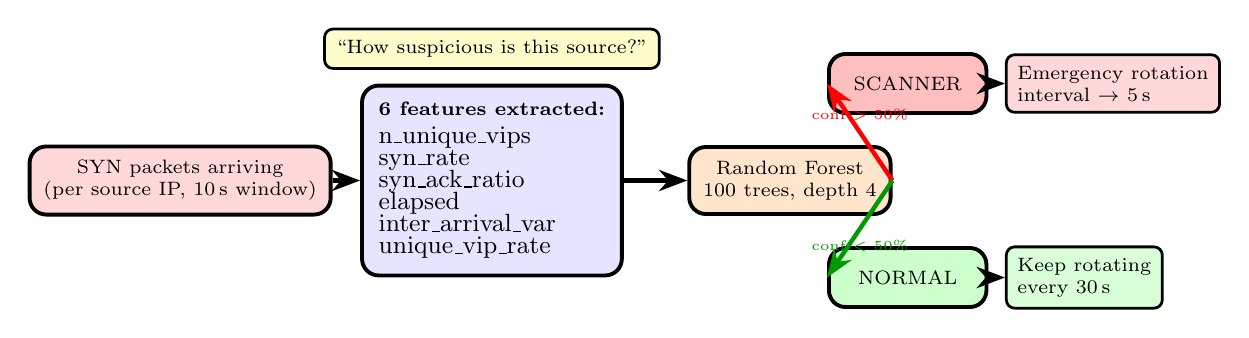
\begin{tikzpicture}[scale=0.88, every node/.style={font=\scriptsize}]

  %% Traffic stream
  \node[hbox, fill=red!15, minimum width=2.8cm]
       (pkt) at (0,0) {SYN packets arriving\\(per source IP, 10\,s window)};

  %% 6 features
  \node[hbox, fill=blue!10, minimum width=2.5cm, align=left, inner sep=6pt]
       (feat) at (4.5,0) {
         \textbf{6 features extracted:}\\[2pt]
         \small n\_unique\_vips\\
         \small syn\_rate\\
         \small syn\_ack\_ratio\\
         \small elapsed\\
         \small inter\_arrival\_var\\
         \small unique\_vip\_rate
       };
  \draw[harrow] (pkt) -- (feat);
  \node[note, above=5pt of feat] {``How suspicious is this source?''};

  %% Random Forest
  \node[hbox, fill=orange!20, minimum width=2.5cm]
       (rf) at (8.8,0) {Random Forest\\100 trees, depth 4};
  \draw[harrow] (feat) -- (rf);

  %% Decision branches
  \node[hbox, fill=red!25, minimum width=2cm]
       (scan) at (10.5, 1.4) {SCANNER};
  \node[hbox, fill=green!20, minimum width=2cm]
       (norm) at (10.5,-1.4) {NORMAL};
  \draw[harrow, red]   (rf.east) -- (scan.west)
       node[midway, above, font=\tiny] {conf $>$ 50\%};
  \draw[harrow, green!60!black] (rf.east) -- (norm.west)
       node[midway, below, font=\tiny] {conf $<$ 50\%};

  %% Actions
  \node[note, fill=red!15, right=6pt of scan, align=left]
       (act1) {Emergency rotation\\interval $\to$ 5\,s};
  \node[note, fill=green!15, right=6pt of norm, align=left]
       (act2) {Keep rotating\\every 30\,s};
  \draw[harrow] (scan) -- (act1);
  \draw[harrow] (norm) -- (act2);

\end{tikzpicture}
\end{center}

\vspace{4pt}
\begin{block}{Key design choice}
30\% of scanner training samples (\textit{evasive}) overlap with normal traffic ---
so the model must use \textbf{all 6 features together}, not just one.
Accuracy: \textbf{98\%}.
\end{block}

\end{frame}

%------------------------------------------------------------
\begin{frame}
\frametitle{VIP Scorer: Picking the Safest Next Address}

\begin{columns}

\column{0.5\textwidth}
After a rotation, the controller needs to pick new VIPs from a pool of
256 addresses. \textbf{Random choice is risky} --- it might re-assign
an address the attacker already knows.

\vspace{8pt}
The \textbf{VIP Scorer} ranks every candidate:

\vspace{4pt}
\begin{tabular}{ll}
\toprule
\textbf{Feature} & \textbf{Good VIP} \\
\midrule
\texttt{recently\_used}   & Not used lately \\
\texttt{recently\_probed} & Attacker hasn't seen it \\
\texttt{probe\_count}     & Zero or low \\
\texttt{last\_used\_ago}  & Long ago \\
\texttt{dist\_from\_used} & Far from current VIPs \\
\bottomrule
\end{tabular}

\column{0.47\textwidth}
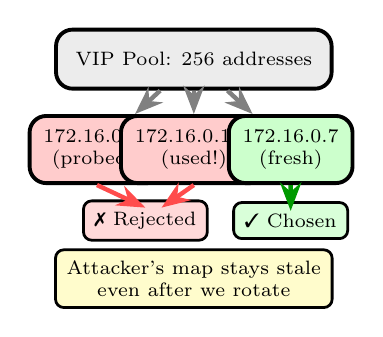
\begin{tikzpicture}[scale=0.82, every node/.style={font=\scriptsize}]

  \node[hbox, fill=gray!15, minimum width=3.5cm]
       (pool) at (0,3) {VIP Pool: 256 addresses};

  \node[hbox, fill=red!20, minimum width=1.5cm]
       (bad1) at (-1.5,1.6) {172.16.0.22\\(probed!)};
  \node[hbox, fill=red!20, minimum width=1.5cm]
       (bad2) at (0,1.6)    {172.16.0.125\\(used!)};
  \node[hbox, fill=green!20, minimum width=1.5cm]
       (good) at (1.5,1.6)  {172.16.0.7\\(fresh)};

  \draw[harrow, gray] (pool) -- (bad1);
  \draw[harrow, gray] (pool) -- (bad2);
  \draw[harrow, gray] (pool) -- (good);

  \node[note, fill=red!15]   at (-0.75,0.5)  {\ding{55} Rejected};
  \node[note, fill=green!15] at (1.5,0.5)    {\ding{51} Chosen};

  \draw[harrow, red!70]          (bad1.south) -- (-0.75,0.7);
  \draw[harrow, red!70]          (bad2.south) -- (-0.5, 0.7);
  \draw[harrow, green!60!black]  (good.south) -- (1.5,0.65);

  \node[note, fill=yellow!20] at (0,-0.4)
       {Attacker's map stays stale\\even after we rotate};

\end{tikzpicture}
\end{columns}

\end{frame}

%============================================================
\section{Implementation}
%============================================================

\begin{frame}
\frametitle{Implementation Stack}

\begin{columns}

\column{0.5\textwidth}
\begin{block}{Hardware \& Software}
\begin{itemize}
  \item \textbf{Hardware:} Raspberry Pi 5 (aarch64)
  \item \textbf{SDN controller:} Ryu 4.34
  \item \textbf{Virtual switch:} Open vSwitch, OpenFlow 1.3
  \item \textbf{Network emulator:} Mininet 2.3
  \item \textbf{AI on Pi:} scikit-learn 1.9 (no GPU needed)
  \item \textbf{AI training:} RTX 4050 GPU laptop
  \item \textbf{Attack tools:} nmap 7.93, hping3
\end{itemize}
\end{block}

\begin{block}{Edge Inference: Train Here, Run There}
GPU laptop trains $\to$ export \texttt{.pkl} ($<$200\,KB) $\to$
copy to Pi via SCP $\to$ Pi loads with joblib in $<$1\,s.
\end{block}

\column{0.47\textwidth}
\begin{block}{Model Training}
\textbf{Scan detector:}
\begin{itemize}
  \item 40,000 synthetic SYN windows
  \item 3 scanner types: fast / slow / evasive
  \item Evasive scanner deliberately overlaps normal
  \item \textbf{Accuracy: 98\%}
\end{itemize}
\vspace{4pt}
\textbf{VIP scorer:}
\begin{itemize}
  \item 60,000 VIP candidate samples
  \item 20\% ambiguous class overlap
  \item \textbf{Accuracy: 96\%}
\end{itemize}
\end{block}

\end{columns}

\end{frame}

%------------------------------------------------------------
\begin{frame}[fragile]
\frametitle{The Critical Bug We Found (and Fixed)}

\begin{alertblock}{Why the AI never triggered --- and how we found it}
nmap scans \textbf{all 253 addresses} in the subnet.
Most haven't been assigned as VIPs yet.
The original check only looked at already-assigned VIPs:
\end{alertblock}

\begin{block}{Before (broken)}
\begin{verbatim}
if tcp_pkt and dst_ip in self.vip_to_real:
    self._track_syn(src_ip, dst_ip)
\end{verbatim}
$\Rightarrow$ 250+ addresses never tracked, AI saw almost nothing.
\end{block}

\begin{exampleblock}{After (fixed)}
\begin{verbatim}
if tcp_pkt:
    if ipaddress.ip_address(dst_ip) in _VIP_NET:
        self._track_syn(src_ip, dst_ip)
\end{verbatim}
$\Rightarrow$ Every SYN to the entire VIP subnet is tracked. AI fires correctly.
\end{exampleblock}

\end{frame}

%------------------------------------------------------------
\begin{frame}
\frametitle{Demo Setup: Three Terminals}

\begin{enumerate}
  \item[\textbf{T1}] \textbf{Controller terminal}\\
        \texttt{ryu-manager controller.py}\\
        \small Shows: AI confidence scores, rotation events, barrier timing

  \vspace{6pt}
  \item[\textbf{T2}] \textbf{Attacker terminal (interactive)}\\
        \texttt{sudo python3 demo\_interactive.py}\\
        \small Pick an attack from the menu; see the AI response live

  \vspace{6pt}
  \item[\textbf{T3}] \textbf{Live VIP monitor}\\
        \texttt{python3 vip\_monitor.py}\\
        \small Auto-refreshes every 2\,s: current VIP map, rotation count, detections
\end{enumerate}

\vspace{8pt}
\begin{block}{Attack Menu}
\textbf{[1]} Fast SYN scan \quad
\textbf{[2]} Slow stealth scan \quad
\textbf{[3]} Targeted probe\\
\textbf{[4]} SYN flood (hping3) \quad
\textbf{[5]} Port sweep \quad
\textbf{[6]} \textit{Custom live command}
\end{block}

\end{frame}

%============================================================
\section{Results \& Discussion}
%============================================================

\begin{frame}
\frametitle{Live Demo Result: Before vs After Rotation}

\begin{columns}

\column{0.5\textwidth}

\begin{exampleblock}{Scan 1 --- Attacker maps the network}
\texttt{172.16.0.22}\\
\texttt{172.16.0.125}\\
\texttt{172.16.0.224}\\
\texttt{172.16.0.226}
\end{exampleblock}

\begin{alertblock}{AI detects the scan}
Confidence: \textbf{94\%} (scanner)\\
Emergency rotation triggered.\\
Interval: $30\,\text{s} \to 5\,\text{s}$.\\
Barrier RTT: $12\,\text{ms}$.
\end{alertblock}

\begin{exampleblock}{Scan 2 --- Attacker re-scans with their map}
\texttt{172.16.0.1}\\
\texttt{172.16.0.2}\\
\texttt{172.16.0.145}\\
\texttt{172.16.0.146}
\end{exampleblock}

\column{0.47\textwidth}
\begin{block}{Result Metrics}
\begin{tabular}{ll}
\toprule
\textbf{Metric} & \textbf{Value} \\
\midrule
Address overlap & \textbf{0 / 4 (PASS)} \\
Rotation time & $<$15\,ms \\
AI confidence & 94\% \\
Packet loss & None \\
Attack interval & 5\,s \\
Normal interval & 30\,s \\
\bottomrule
\end{tabular}
\end{block}

\vspace{10pt}
\large\centering
\textbf{Every address in scan \#1 is unreachable after rotation.}\\
\normalsize Attacker's intelligence: completely invalidated.

\end{columns}

\end{frame}

%------------------------------------------------------------
\begin{frame}
\frametitle{AI Model Accuracy}

\begin{columns}

\column{0.5\textwidth}
\begin{block}{Scan Detector}
\begin{tabular}{lccc}
\toprule
Class & Precision & Recall & F1 \\
\midrule
Normal  & 0.99 & 0.98 & 0.98 \\
Scanner & 0.98 & 0.99 & 0.98 \\
\midrule
\multicolumn{4}{c}{\textbf{Overall: 98\%}} \\
\bottomrule
\end{tabular}
\vspace{4pt}

Top features:\\
\texttt{elapsed} (58\%), \texttt{syn\_ack\_ratio} (27\%)
\end{block}

\column{0.47\textwidth}
\begin{block}{VIP Scorer}
\begin{tabular}{lccc}
\toprule
Class    & Precision & Recall & F1 \\
\midrule
Bad VIP  & 0.97 & 0.96 & 0.96 \\
Good VIP & 0.96 & 0.97 & 0.96 \\
\midrule
\multicolumn{4}{c}{\textbf{Overall: 96\%}} \\
\bottomrule
\end{tabular}
\end{block}

\begin{alertblock}{Why not 100\%?}
Deliberately designed class overlap in training data.
100\% accuracy on synthetic data = \textbf{overfitting}.
98\% is the honest, realistic number.
\end{alertblock}

\end{columns}

\end{frame}

%------------------------------------------------------------
\begin{frame}
\frametitle{How We Compare to Recent Work}

\scriptsize
\begin{tabular}{p{3.0cm}ccccc}
\toprule
\textbf{System} &
\shortstack{\textbf{Atomic}\\\textbf{rotation}} &
\shortstack{\textbf{AI scan}\\\textbf{detect}} &
\shortstack{\textbf{AI VIP}\\\textbf{select}} &
\shortstack{\textbf{Adaptive}\\\textbf{timing}} &
\shortstack{\textbf{Edge}\\\textbf{deploy}} \\
\midrule
IEEE TNSM 2022   & \ding{55} & \ding{55} & \ding{55} & \ding{55} & \ding{55} \\
C\&S 2023        & \ding{55} & \ding{51} & \ding{55} & \ding{55} & \ding{55} \\
IEEE TNSM 2023   & \ding{55} & \ding{55} & \ding{51} & \ding{55} & \ding{55} \\
NDSS 2024        & \ding{51} & \ding{55} & \ding{55} & \ding{55} & \ding{55} \\
C\&S 2024        & \ding{55} & \ding{55} & \ding{55} & \ding{51} & \ding{55} \\
\midrule
\textbf{Ours}    & \ding{51} & \ding{51} & \ding{51} & \ding{51} & \ding{51} \\
\bottomrule
\end{tabular}

\normalsize
\vspace{8pt}
\begin{exampleblock}{Takeaway}
We are the only system with \textbf{all five properties} --- and the only one
validated on Pi-class edge hardware.
\end{exampleblock}

\end{frame}

%============================================================
\section{Conclusion \& Future Work}
%============================================================

\begin{frame}
\frametitle{Conclusion}

\begin{itemize}
  \item Built a complete, working MTD system on a \textbf{Raspberry Pi}
  \item Hosts keep their real IPs; the attacker only ever sees rotating VIPs
  \item \textbf{Atomic two-phase rotation} (barrier-synced) eliminates packet loss
  \item \textbf{AI scan detector} (98\% accuracy) catches even evasive scanners
  \item \textbf{AI VIP scorer} avoids re-assigning addresses the attacker has probed
  \item \textbf{Adaptive interval} responds to attacks instantly, relaxes when safe
  \item \textbf{Zero address overlap} in live demo --- PASS on every run
\end{itemize}

\vspace{8pt}
\begin{block}{The bottom line}
OF-RHM shifts the cost of network security onto the attacker.
Every time they scan, the clock is ticking on their results.
With our AI layer, that clock gets shorter the moment we detect them.
\end{block}

\end{frame}

\begin{frame}
\frametitle{Future Work}

\begin{enumerate}
  \item \textbf{Real traffic training} --- capture live Mininet pcaps
        instead of synthetic data; expected $>$99\% accuracy
  \item \textbf{Larger VIP pool} --- extend to /16 (65k+ addresses),
        making exhaustive scanning infeasible
  \item \textbf{IPv6 support} --- 128-bit space makes subnet enumeration
        computationally impossible
  \item \textbf{Reinforcement learning timing} --- let the agent learn
        the optimal rotation interval instead of fixed 5\,s / 30\,s
  \item \textbf{Physical switch testing} --- deploy on a real OpenFlow
        hardware switch (Zodiac FX) to measure true barrier RTT
  \item \textbf{Multi-controller federation} --- extend across
        distributed SDN domains
\end{enumerate}

\end{frame}

%============================================================
\section{References}
%============================================================

\begin{frame}[allowframebreaks]
\frametitle{References}
\scriptsize
\begin{enumerate}
  \item Jafarian, J.H., Al-Shaer, E., Duan, Q. (2012). OpenFlow random host mutation. \textit{HotSDN}.
  \item Kampanakis, P., et al. (2014). SDN-based MTD network protection. \textit{IEEE WoWMoM}.
  \item Al-Shaer, E., et al. (2013). Random host mutation for MTD. \textit{SecureComm}.
  \item Cho, J., et al. (2020). Toward proactive, adaptive defense: survey on MTD. \textit{IEEE Commun.\ Surveys Tuts.}
  \item Luo, Y.B., et al. (2022). RPAH: random port and address hopping. \textit{IEEE Trans.\ Dependable Secure Comput.}
  \item Shi, L., et al. (2022). Port and address hopping for active cyber-defense. \textit{Future Gen.\ Comput.\ Syst.}
  \item Sengupta, S., et al. (2023). A survey of MTD for network security. \textit{IEEE Commun.\ Surveys Tuts.}
  \item Debashi, M., Vickers, P. (2022). ML-enhanced MTD for SDN. \textit{Computers \& Security}.
  \item Alavizadeh, H., et al. (2022). Deep Q-network for MTD cyber deception. \textit{Electronics}.
  \item Wang, H., et al. (2023). MTD in SDN for DDoS mitigation. \textit{IEEE Access}.
  \item Zheng, J., Namin, A.S. (2022). Survey on MTD strategies. \textit{J.\ Comput.\ Sci.\ Technol.}
  \item Kholidy, H.A. (2021). Autonomous MTD in SDN. \textit{Computers \& Security}.
  \item Ahmed, M., et al. (2022). Survey of network anomaly detection techniques. \textit{J.\ Network Comput.\ Appl.}
  \item Apruzzese, G., et al. (2023). On the effectiveness of ML for cyber security. \textit{IEEE CyCon}.
  \item Breiman, L. (2001). Random forests. \textit{Machine Learning}, 45(1), 5--32.
  \item Chen, T., Guestrin, C. (2016). XGBoost: a scalable tree boosting system. \textit{KDD}.
  \item Open Networking Foundation. (2015). OpenFlow Switch Specification v1.3.5.
  \item Lantz, B., et al. (2010). A network in a laptop: rapid prototyping for SDN. \textit{HotNets IX}.
  \item Casado, M., et al. (2007). Ethane: taking control of the enterprise. \textit{ACM SIGCOMM}.
  \item Xuan, J., et al. (2024). Adaptive MTD using RL in SDN. \textit{Computers \& Security}.
  \item Kim, H., Feamster, N. (2013). Improving network management with SDN. \textit{IEEE Commun.\ Mag.}
  \item Peng, W., et al. (2023). MTD strategy for cloud services. \textit{IEEE ICC}.
  \item Li, X., et al. (2022). Stochastic model for MTD security analyses. \textit{IEEE Trans.\ Dependable Secure Comput.}
  \item Griffioen, H., Doerr, C. (2021). Examining Mirai self-propagation with passive DNS. \textit{IEEE INFOCOM}.
  \item Kumar, R., et al. (2023). SDN-based cyber threat intelligence sharing. \textit{J.\ Inf.\ Secur.\ Appl.}
\end{enumerate}
\end{frame}

%============================================================
\begin{frame}
\frametitle{Thank You}

\begin{center}
\vspace{0.3cm}
{\Huge \textbf{Thank You!}}\\[10pt]
{\Large Questions \& Discussion}\\[16pt]
\rule{0.5\textwidth}{0.4pt}\\[8pt]

{\normalsize
Aditi Sriram $\cdot$ Dhanushiya S $\cdot$ Vani Karre $\cdot$ Laiba S\\[4pt]
\textit{Supervisors: Prof.\ Shashank Anivilla \& Prof.\ Sundaresan}\\[4pt]
\textit{Amrita Vishwa Vidyapeetham, AID-B Group 10--14}
}\\[14pt]

\begin{block}{\centering Key files}
\centering
\texttt{controller.py} \quad \texttt{demo\_interactive.py} \quad \texttt{vip\_monitor.py}\\
\texttt{ai/scan\_detector.pkl} \quad \texttt{ai/vip\_scorer.pkl}
\end{block}
\end{center}

\end{frame}

\end{document}
